\documentclass{standalone}
\usepackage{tikz}
\usetikzlibrary{patterns, positioning}
\usepackage[sfdefault]{ClearSans} %% option 'sfdefault' activates Clear Sans as the default text font
\usepackage[T1]{fontenc}

\begin{document}
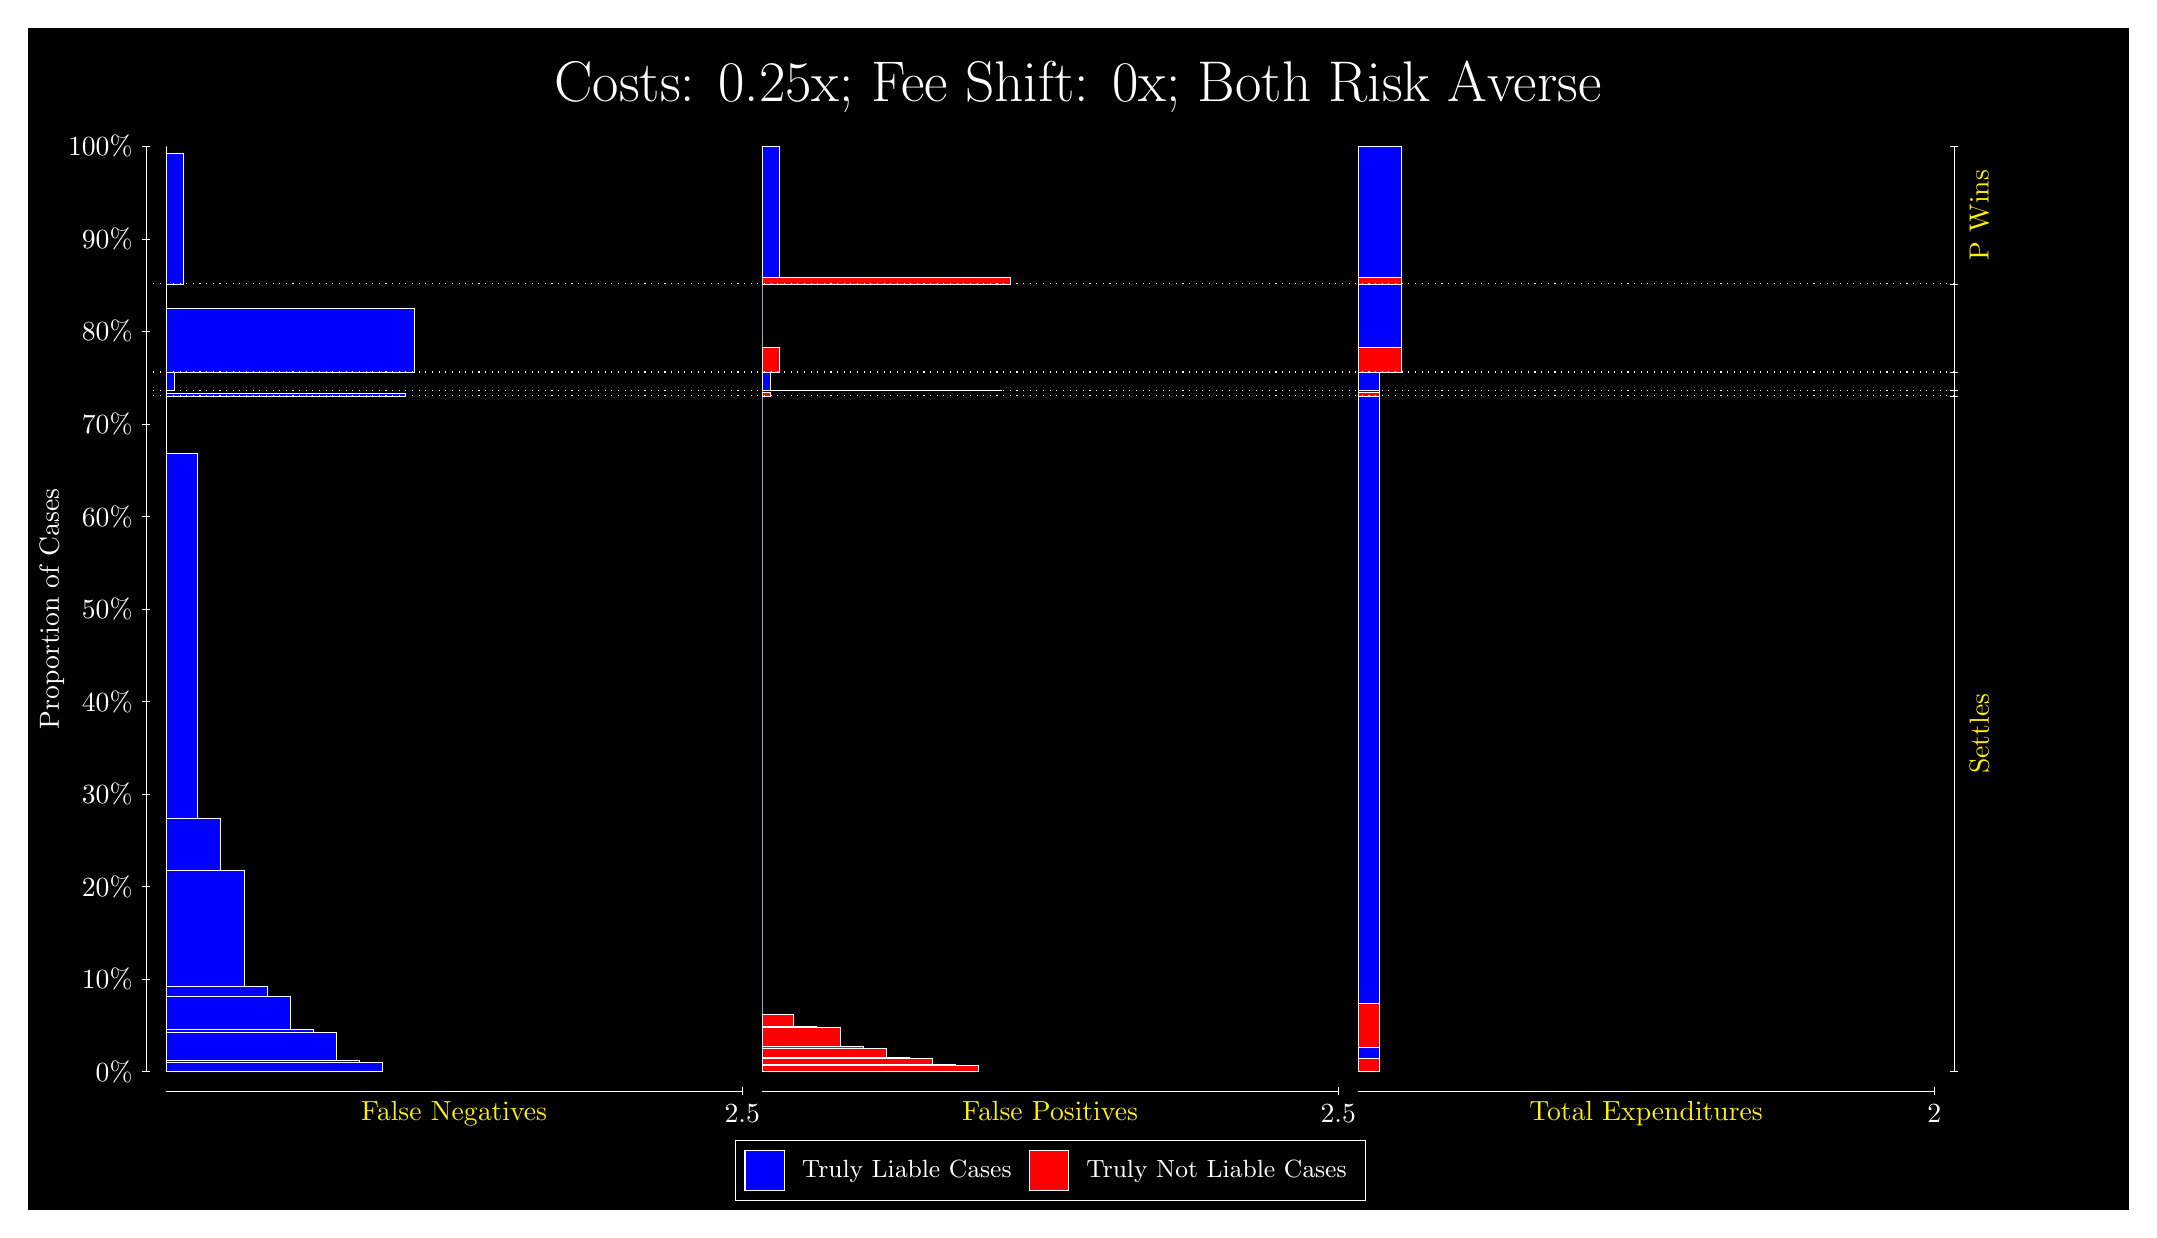
\begin{tikzpicture}
\draw[fill=black] (0,0) rectangle (26.667,15);
\draw[text=white] (0,13.5) rectangle (26.667,15) node[midway] {\huge Costs: 0.25x; Fee Shift: 0x; Both Risk Averse};
\draw[white, very thin] (1.5,1.75) -- (1.5,13.5);
\node[rotate=90, text=white, anchor=center] at (0.3, 7.625) {Proportion of Cases};
\draw[white, very thin] (1.45,1.75) -- (1.55,1.75);
\node[text=white, anchor=east] at (1.45, 1.75) {0\%};
\draw[white, very thin] (1.45,2.925) -- (1.55,2.925);
\node[text=white, anchor=east] at (1.45, 2.925) {10\%};
\draw[white, very thin] (1.45,4.1) -- (1.55,4.1);
\node[text=white, anchor=east] at (1.45, 4.1) {20\%};
\draw[white, very thin] (1.45,5.275) -- (1.55,5.275);
\node[text=white, anchor=east] at (1.45, 5.275) {30\%};
\draw[white, very thin] (1.45,6.45) -- (1.55,6.45);
\node[text=white, anchor=east] at (1.45, 6.45) {40\%};
\draw[white, very thin] (1.45,7.625) -- (1.55,7.625);
\node[text=white, anchor=east] at (1.45, 7.625) {50\%};
\draw[white, very thin] (1.45,8.8) -- (1.55,8.8);
\node[text=white, anchor=east] at (1.45, 8.8) {60\%};
\draw[white, very thin] (1.45,9.975) -- (1.55,9.975);
\node[text=white, anchor=east] at (1.45, 9.975) {70\%};
\draw[white, very thin] (1.45,11.15) -- (1.55,11.15);
\node[text=white, anchor=east] at (1.45, 11.15) {80\%};
\draw[white, very thin] (1.45,12.325) -- (1.55,12.325);
\node[text=white, anchor=east] at (1.45, 12.325) {90\%};
\draw[white, very thin] (1.45,13.5) -- (1.55,13.5);
\node[text=white, anchor=east] at (1.45, 13.5) {100\%};

\draw[white, very thin] (24.457,1.75) -- (24.457,13.5);
\draw[white, very thin] (24.407,1.75) -- (24.507,1.75);
\node[anchor=west] at (24.407, 1.75) {};
\draw[white, very thin] (24.407,10.331) -- (24.507,10.331);
\node[anchor=west] at (24.407, 10.331) {};
\draw[white, very thin] (24.407,10.404) -- (24.507,10.404);
\node[anchor=west] at (24.407, 10.404) {};
\draw[white, very thin] (24.407,10.634) -- (24.507,10.634);
\node[anchor=west] at (24.407, 10.634) {};
\draw[white, very thin] (24.407,11.753) -- (24.507,11.753);
\node[anchor=west] at (24.407, 11.753) {};
\draw[white, very thin] (24.407,13.5) -- (24.507,13.5);
\node[anchor=west] at (24.407, 13.5) {};

\draw[white, very thin, fill=blue] (1.75,1.75) rectangle (4.4946,1.87);
\draw[white, very thin, fill=blue] (1.75,1.87) rectangle (4.2018,1.8872);
\draw[white, very thin, fill=blue] (1.75,1.8872) rectangle (3.9091,2.2453);
\draw[white, very thin, fill=blue] (1.75,2.2453) rectangle (3.6163,2.2831);
\draw[white, very thin, fill=blue] (1.75,2.2831) rectangle (3.3236,2.7034);
\draw[white, very thin, fill=blue] (1.75,2.7034) rectangle (3.0308,2.831);
\draw[white, very thin, fill=blue] (1.75,2.831) rectangle (2.738,4.3062);
\draw[white, very thin, fill=blue] (1.75,4.3062) rectangle (2.4453,4.9717);
\draw[white, very thin, fill=blue] (1.75,4.9717) rectangle (2.1525,9.6032);
\draw[white, very thin, fill=red] (1.75,9.6032) rectangle (1.75,10.331);
\draw[white, very thin, fill=blue] (1.75,10.331) rectangle (4.7873,10.359);
\draw[white, very thin, fill=red] (1.75,10.359) rectangle (1.75,10.404);
\draw[white, very thin, fill=blue] (1.75,10.404) rectangle (1.8598,10.631);
\draw[white, very thin, fill=red] (1.75,10.631) rectangle (1.75,10.634);
\draw[white, very thin, fill=blue] (1.75,10.634) rectangle (4.8971,11.444);
\draw[white, very thin, fill=red] (1.75,11.444) rectangle (1.75,11.753);
\draw[white, very thin, fill=blue] (1.75,11.753) rectangle (1.9696,13.411);
\draw[white, very thin, fill=red] (1.75,13.411) rectangle (1.75,13.5);
\draw[white, very thin, fill=red] (9.3189,1.75) rectangle (12.063,1.8261);
\draw[white, very thin, fill=red] (9.3189,1.8261) rectangle (11.771,1.8366);
\draw[white, very thin, fill=red] (9.3189,1.8366) rectangle (11.478,1.924);
\draw[white, very thin, fill=red] (9.3189,1.924) rectangle (11.185,1.9365);
\draw[white, very thin, fill=red] (9.3189,1.9365) rectangle (10.892,2.0513);
\draw[white, very thin, fill=red] (9.3189,2.0513) rectangle (10.6,2.0679);
\draw[white, very thin, fill=red] (9.3189,2.0679) rectangle (10.307,2.3094);
\draw[white, very thin, fill=red] (9.3189,2.3094) rectangle (10.014,2.3271);
\draw[white, very thin, fill=red] (9.3189,2.3271) rectangle (9.7214,2.4779);
\draw[white, very thin, fill=blue] (9.3189,2.4779) rectangle (9.3189,10.331);
\draw[white, very thin, fill=red] (9.3189,10.331) rectangle (9.4287,10.377);
\draw[white, very thin, fill=blue] (9.3189,10.377) rectangle (9.3189,10.404);
\draw[white, very thin, fill=red] (9.3189,10.404) rectangle (12.356,10.407);
\draw[white, very thin, fill=blue] (9.3189,10.407) rectangle (9.4287,10.634);
\draw[white, very thin, fill=red] (9.3189,10.634) rectangle (9.5384,10.943);
\draw[white, very thin, fill=blue] (9.3189,10.943) rectangle (9.3189,11.753);
\draw[white, very thin, fill=red] (9.3189,11.753) rectangle (12.466,11.843);
\draw[white, very thin, fill=blue] (9.3189,11.843) rectangle (9.5384,13.5);
\draw[white, very thin, fill=red] (16.888,1.75) rectangle (17.162,1.9185);
\draw[white, very thin, fill=blue] (16.888,1.9185) rectangle (17.162,2.0557);
\draw[white, very thin, fill=red] (16.888,2.0557) rectangle (17.162,2.6151);
\draw[white, very thin, fill=blue] (16.888,2.6151) rectangle (17.162,10.331);
\draw[white, very thin, fill=red] (16.888,10.331) rectangle (17.162,10.377);
\draw[white, very thin, fill=blue] (16.888,10.377) rectangle (17.162,10.404);
\draw[white, very thin, fill=red] (16.888,10.404) rectangle (17.162,10.407);
\draw[white, very thin, fill=blue] (16.888,10.407) rectangle (17.162,10.634);
\draw[white, very thin, fill=red] (16.888,10.634) rectangle (17.437,10.943);
\draw[white, very thin, fill=blue] (16.888,10.943) rectangle (17.437,11.753);
\draw[white, very thin, fill=red] (16.888,11.753) rectangle (17.437,11.843);
\draw[white, very thin, fill=blue] (16.888,11.843) rectangle (17.437,13.5);
\draw[white, dotted] (1.5,10.331) -- (24.457,10.331);
\draw[white, dotted] (1.5,10.404) -- (24.457,10.404);
\draw[white, dotted] (1.5,10.634) -- (24.457,10.634);
\draw[white, dotted] (1.5,11.753) -- (24.457,11.753);
\draw[white, very thin] (1.75,1.5) -- (9.0689,1.5);
\node[text=yellow, anchor=north] at (5.4094, 1.5) {False Negatives};
\draw[white, very thin] (9.0689,1.45) -- (9.0689,1.55);
\node[text=white, anchor=north] at (9.0689, 1.45) {2.5};

\draw[white, very thin] (9.3189,1.5) -- (16.638,1.5);
\node[text=yellow, anchor=north] at (12.978, 1.5) {False Positives};
\draw[white, very thin] (16.638,1.45) -- (16.638,1.55);
\node[text=white, anchor=north] at (16.638, 1.45) {2.5};

\draw[white, very thin] (16.888,1.5) -- (24.207,1.5);
\node[text=yellow, anchor=north] at (20.547, 1.5) {Total Expenditures};
\draw[white, very thin] (24.207,1.45) -- (24.207,1.55);
\node[text=white, anchor=north] at (24.207, 1.45) {2};

\node[text=yellow, centered, rotate=90] at (24.777, 6.0405) {Settles};



\node[text=yellow, centered, rotate=90] at (24.777, 12.627) {P Wins};

\draw (12.978300999999998,1.5) node[draw=none] (baseCoordinate) {};
\begin{scope}[align=center]
        \matrix[scale=0.5, draw=white, below=0.5cm of baseCoordinate, nodes={draw}, column sep=0.1cm]{
            \node[rectangle, draw, minimum width=0.5cm, minimum height=0.5cm, fill=blue] {}; &
            \node[draw=none, font=\small, text=white] (B) {Truly Liable Cases}; &
            \node[rectangle, draw, minimum width=0.5cm, minimum height=0.5cm, fill=red] {}; &
            \node[draw=none, font=\small, text=white] (B) {Truly Not Liable Cases}; \\
            };
\end{scope}

\end{tikzpicture}
\end{document}